\chapter{Frontend-Suche}

Dieses Kapitel handelt von der Implementierung der Frontend-Suche des Projektes in Elasticsearch. Im ersten Schritt wird die Suche und die automatische Vervollständigung übertragen. Danach sollen noch eine neue Suchart, welche mehr Felder umfasst, sowie eine Anzeige der Autoren, welche bei der aktuellen Suche die meisten Artikel verfasst haben.

\section{Indexierung}

Um die Daten zu indexieren, wurde eine statische Code-Analyse durchgeführt, welche Daten aktuell als Suchergebnis angezeigt werden. Dafür wird der gesamte Code zur Suche untersucht und alle Werte aufgeschrieben. Aufgrund dieser Basis wurde eine Abfrage konstruiert, welche alle Daten an den Aggregat-Filter weiterreicht. Dann werden diese aggregiert, wie schon im letzten Kapitel beschrieben, und auch transformiert. So wird zum Beispiel eine URL, welche vorher immer zur Laufzeit zusammengesetzt wurde direkt schon zusammengebaut in die Suchmaschine eingepflegt. 

Für die Auto-Vervollständigung mussten auch neue Felder angelegt werden. Es gibt im Projekt für jede Suchart eine eigene Vervollständigung. Um dies auch im Index abzubilden, wurden diverse Vervollständigungs-Felder angelegt, welche zum Teil einzelne Felder oder Feldmengen durchsuchen. Diese Felder wurden dann mithilfe des Aggregat-Filters befüllt. Ein Beispiel:

Der Titel eines Artikels und die dazugehörige Sigle werden in zwei unterschiedlichen Felder gespeichert. Sie sollten allerdings für die Vervollständigung zusammengebaut werden. Dafür wird in dem Aggregationsfilter von Logstash definiert, dass dieses Feld zusammengebaut werden soll:

\begin{lstlisting}[language=PHP, frame=single, label={lst:stringConcat}, caption=Zeichenketten-Konkatination im Aggregat Filter von Logstash ,captionpos=b] 
map['artikel_titel_suggest'] ||= 
    '['+event.get('lemma_bezeichnung').to_s+']'
        +event.get('artikel_titel').to_s
\end{lstlisting}
    
Die daraus entstandene Zeichenkette wird in das Suggestions-Feld von Elasticsearch gegeben. Elasticsearch indexiert daraufhin die Zeichenkette so, dass jedes Wort zur Auto-Vervollständigung benutzt werden kann, allerdings als Ausgabe immer die komplette Zeichenkette zurückgegeben wird.

Sollten aus einem Datensatz mehrere Felder indexiert werden, ist es möglich, auch ein Array von Daten an das Auto-Vervollständigungsfeld von Elasticsearch weiterzugeben.

Der Index ist hierbei der aktuell Größte im DietrichOnline-Projekt mit rund 1.4 Millionen Einträgen. Die aktuelle Größe des Indexes zusammen mit den Feldern zur Auto-Vervollständigung beläuft sich auf rund 4.2 Gigabyte. 

Durch die Definition der Feldtypen wurde die Größe des Index schon ein wenig reduziert. So wurde zum Beispiel die URL nur als Zeichenkette und nicht als Volltext gespeichert. Normalerweise werden Felder, die unter 255 Zeichen lang sind, als Keyword und Volltext gleichzeitig indexiert. Um diese doppelte Indexierung zu verhindern wurde sich für einen Typen entschieden.

Beim ersten Lauf der Pipeline, kam es zu einem Absturz von Logstash. Dies lag daran, dass Logstash nicht genügend Speicher hatte, um diese Abfrage abzuarbeiten. Um weitere Probleme von dieser Seite zu verhindern, wurde der RAM für Logstash auf 4 Gigabyte erhöht.

\section{Integration}

\subsection{Paginierung}

Die bisherige Paginierung holte bis zu 1001 Ergebnisse aus der Datenbank und generierte daraufhin die Paginierung. Die Begrenzung ergibt sich daher, dass die vollen Datensätze aus der Datenbank geholt wurden, und dies bei größeren Zahlen zu einer langen Laufzeit führte.

Diese Einschränkung kann durch den Einsatz von Elasticsearch als Suchmaschine entfernt werden. Dazu wird eine Abfrage abgesetzt, die alle Ergebnisse zählt. Für diesen Fall liefert Elasticsearch eine Count-Abfrage mit.

Durch diesen wird eine Paginierung generiert. Dafür wird mithilfe der Seitennummer ein Offset für die Abfrage generiert, sodass Elasticsearch immer nur die aktuellen Ergebnisse für die Suche liefert.

\begin{lstlisting}[language=PHP, frame=single, label={lst:generierung},  caption=Generierung des Offsets für die Paginierung,captionpos=b] 
$result = $repo->findUserSearchResult(
    //array with all search-querys and junctors
    $this->userSearchItemArray, 
    //offset for the results
    ($request->query->getInt('pageNumber', 1) * 30 - 30)
);
\end{lstlisting}

\subsection{Query String}
Um verschiedene Sucharten zu unterstüzen, wurde eine Suche mittels Query-String verwendet, da diese erlaubt, Wildcard-Symbole zu verwenden. Dadurch ergeben sich zwar Performanz-Einbußen, allerdings sind Wildcard-Suchen ein oft genutztes Element in diesem Projekt und daher erforderlich.

\begin{lstlisting}[language=PHP, frame=single, label={lst:aufbauQueryString}, caption=Beispiel eines Query-Strings,captionpos=b] 
$subQuery = [
    'query_string' => [
        'query' => $userSearchItem->getValue(),
        'fields' => [
            "artikel_titel",
            "lemma_bezeichnung",
            [...], //weitere Felder
            "normlitref_entries.normlitref_kvk_bezeichnung",
        ],
        "lenient" => true,
    ],
];
\end{lstlisting}

Ein Augenmerk muss auch noch auf die Lenient-Option gelegt werden. Ist dieser Wert nicht gesetzt, bricht die Suche mit einem Format-Fehler, wie das Suchen einer Zeichenkette in einem Zahlen-Feld, ab. Diese Funktion wurde daher bei allen Suchen abgeschaltet. Gerade bei diesem Beispiel, muss die Suche Felder mit diversem Inhalten gleichzeitig durchsuchen, ohne abzubrechen. 

\subsection{Boolesche Logik}

Es ist möglich eine boolesche Logik bei der Frontend-Suche im DietrichOnline zu verwenden. Um diese umzusetzen, werden die Teile der Abfrage ineinander verschachtelt \ref{lst:booleanEla}:

\begin{lstlisting}[language=PHP, frame=single, label={lst:booleanEla}, caption=Auschnitt aus der boolischen Logik für das DietrichOnline-Projekt,captionpos=b] 
switch ($userSearchItem->getJunktor()) {
    case UserSearchItem::JUNKTOR_NO: //First Entry
        $this->fullQuery = [
            'bool' => [
                'must' => [
                    $this->addTypeValue($userSearchItem), //Add Search
                ],
            ],
        ];
        break;
    case UserSearchItem:: JUNKTOR_AND: //MUST
        $this->fullQuery = [
            'bool' => [
                'must' => [
                    $this->addTypeValue($userSearchItem), //Add Search
                    $this->fullQuery, //First Part of Query
                ],
            ],
        ];
        break;
[...] // More Cases like OR or AND NOT
\end{lstlisting}

Bei jeder Suche wird ein Array mit allen Suchanfragen weitergegeben. Das erste Item im Array hat dabei niemals einen Junktor. Dafür existiert der Fall in Zeile 2-10. Existiert eine weitere Stelle im Array, ist auch ein Junktor mit angegeben. Dieser wird dann in dem unten gezeigten Switch-Case ausgelesen. Dann wird eine weitere Boolean-Abfrage geschrieben, welcher zum einen den neuen Teil der Suche, sowie die bisherige Suche enthält.



\subsection{Auto-Vervollständigung}

Die Indexierung dieser Felder wurde schon im obigen Kapitel besprochen. Hier geht es nun darum, wie eine Abfrage an dieses System aussieht. Damit das System weiß, welches Suggestions-Feld verwendet werden soll, wird dieses in der Applikation als Array hinterlegt. Normalerweise wird auch der gesamte Eintrag mit aus der Datenbank geladen. Da dies bei der Projektstruktur DietrichOnlines nicht benötigt wird, wird das \_source-Feld als leere Zeichenkette gesetzt.


\begin{lstlisting}[language=PHP, frame=single, label={lst:autocompleParams}, caption=Auschnitt aus der Abfrage zur Auto-Vervollständigung,captionpos=b] 
$params = [
    'index' => 'dietrich_frontend',
    'body' => [
        '_source' => '', //Empty Source since we need only the String
        'suggest' => [
            'auto_complete' => [
                'prefix' => $matchAgainst,
                'completion' => [
                    'field' => SEA::AUTOCOMPLETE_COLUMNS[$categoryIndex],
                    'size' => $maxMatches,
                    'skip_duplicates' => true,
]]]]];
\end{lstlisting}

\subsection{Vollständige Suche}

Die vollständige Suche soll die aktuelle Schnellsuche, welche aus Artikeltitel mit Sigle besteht, ersetzen. Dazu wurde zuerst geschaut, welche Felder sonst noch von Interesse sein könnten. 

Nach einer Besprechung mit einem Mitarbeiter wurde eine Liste mit relevanten Spalten erstellt. Daraufhin wurde analysiert, welche Spalten für die Auto-Vervollständigung indexiert werden sollen. Dabei wurden Felder, bei denen es keinen Sinn ergibt, sie automatisch zu vervollständigen, wie das ID-Feld, herausgenommen. Mit den verbleibenden Feldern wurde dann ein Auto-Vervollständigungs-Feld gebaut.

\subsection{Autoren}

Bei jeder Suche soll mit einer Auswertung angereichert werden, welche Autoren in der aktuellen Suche die meisten Artikel verfasst haben. Dazu wird eine Aggregation bei jeder Suche auf dem Autoren-Feld durchgeführt. Die Abfrage wird dafür um einen Parameter erweitert \ref{lst:bestAuthors}:

\begin{lstlisting}[language=PHP, frame=single, label={lst:bestAuthors}, caption=Auschnitt aus der Abfrage zur Aggregation der Autoren,captionpos=b] 
'aggs' => [
    'best_authors' => [
        'terms' => [
            'field' => 'artikel_autor.keyword',
]]],
\end{lstlisting}


Nun wird bei jeder Suchanfrage eine Aggregation namens 'best\_authors' zurück-geliefert. Diese enthält den Namen, sowie die Anzahl der gefundenen Dokumente des Autors in der jeweiligen Suche. 
Mit diesen Daten war es nun möglich, Schaltflächen zu generieren, welche eine neue Suche mit den Autorennamen starten.


\begin{figure}
	\centering
	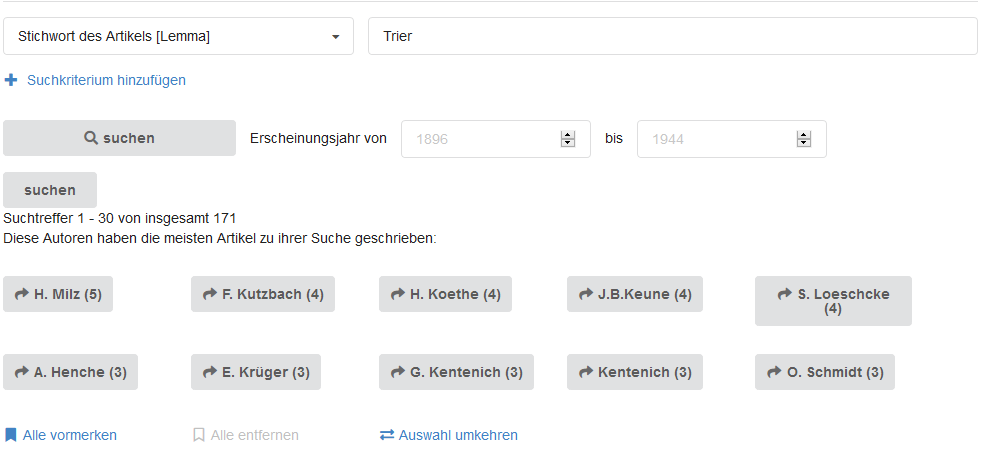
\includegraphics[width=1\linewidth]{images/best_authors.png}
	\caption{Abbildung der erweiterten Suche}
	\label{img:erweiterteSuche}
\end{figure}
